%%%%%%%%%%%%%%%%%%%%%%%%%%%%%%%%%%%%%%%%%
% Journal Article
% LaTeX Template
% Version 1.4 (15/5/16)
%
% This template has been downloaded from:
% http://www.LaTeXTemplates.com
%
% Original author:
% Frits Wenneker (http://www.howtotex.com) with extensive modifications by
% Vel (vel@LaTeXTemplates.com)
%
% License:
% CC BY-NC-SA 3.0 (http://creativecommons.org/licenses/by-nc-sa/3.0/)
%
%%%%%%%%%%%%%%%%%%%%%%%%%%%%%%%%%%%%%%%%%

%----------------------------------------------------------------------------------------
%	PACKAGES AND OTHER DOCUMENT CONFIGURATIONS
%----------------------------------------------------------------------------------------

\documentclass[twoside,twocolumn]{article}

\usepackage{blindtext} % Package to generate dummy text throughout this template 

\usepackage[sc]{mathpazo} % Use the Palatino font
\usepackage[T1]{fontenc} % Use 8-bit encoding that has 256 glyphs
\linespread{1.05} % Line spacing - Palatino needs more space between lines
\usepackage{microtype} % Slightly tweak font spacing for aesthetics

\usepackage[italian]{babel} % Language hyphenation and typographical rules

\usepackage[hmarginratio=1:1,top=32mm,columnsep=20pt]{geometry} % Document margins
\usepackage[hang, small,labelfont=bf,up,textfont=it,up]{caption} % Custom captions under/above floats in tables or figures
\usepackage{booktabs} % Horizontal rules in tables

\usepackage[utf8]{inputenc}

\usepackage{lettrine} % The lettrine is the first enlarged letter at the beginning of the text

\usepackage{enumitem} % Customized lists
\setlist[itemize]{noitemsep} % Make itemize lists more compact

\usepackage{abstract} % Allows abstract customization
\renewcommand{\abstractnamefont}{\normalfont\bfseries} % Set the "Abstract" text to bold
\renewcommand{\abstracttextfont}{\normalfont\small\itshape} % Set the abstract itself to small italic text

\usepackage{titlesec} % Allows customization of titles
\renewcommand\thesection{\Roman{section}} % Roman numerals for the sections
\renewcommand\thesubsection{\roman{subsection}} % roman numerals for subsections
\titleformat{\section}[block]{\large\scshape\centering}{\thesection.}{1em}{} % Change the look of the section titles
\titleformat{\subsection}[block]{\large}{\thesubsection.}{1em}{} % Change the look of the section titles

\usepackage{fancyhdr} % Headers and footers
\pagestyle{fancy} % All pages have headers and footers
\fancyhead{} % Blank out the default header
\fancyfoot{} % Blank out the default footer
\fancyhead[C]{Running title $\bullet$ May 2016 $\bullet$ Vol. XXI, No. 1} % Custom header text
\fancyfoot[RO,LE]{\thepage} % Custom footer text

\usepackage{titling} % Customizing the title section

\usepackage{hyperref} % For hyperlinks in the PDF

\usepackage{graphicx}


%----------------------------------------------------------------------------------------
%	TITLE SECTION
%----------------------------------------------------------------------------------------

\setlength{\droptitle}{-4\baselineskip} % Move the title up

\pretitle{\begin{center}\Huge\bfseries} % Article title formatting
\posttitle{\end{center}} % Article title closing formatting
\title{Sviluppo di un robot Line Follower con l'impiego del microcontrollore Arduino Uno} % Article title
\author{%
\textsc{Davide Cristini}\thanks{A thank you or further information} \\[1ex] % Your name
\normalsize Università Degli Studi dell'Aquila \\ % Your institution
\normalsize \href{mailto:john@smith.com}{john@smith.com} 
\and 
\textsc{Matteo Polsinelli}\thanks{Corresponding author} \\[1ex]
\normalsize Università degli Studi Dell'Aquila \\ 
\normalsize \href{mailto:polsinellimatteo91@gmail.com}{jane@smith.com}
}
\date{\today} % Leave empty to omit a date
\renewcommand{\maketitlehookd}{%
\begin{abstract}
\noindent Durante il corso di Laboratorio di Autoamtica è stato realizzanto un robot in grado di, attraverso dei sensori infrarossi, seguire una linea nera.
\end{abstract}
}

%----------------------------------------------------------------------------------------

\begin{document}

% Print the title
\maketitle

%----------------------------------------------------------------------------------------
%	ARTICLE CONTENTS
%----------------------------------------------------------------------------------------

\section{Introduzione}
Uno dei temi odierni più discussi è quello riguardante nuovi sistemi che siano in grado, autonomamente e senza l'intervento umano, di completare un task assegnato.
C'è molto interesse per questo settore, sia in ambito scientifico ma sopratutto in quello aziendale. 

Nell'industria automobilistica la Tesla Inc è stata l'apri pista per veicoli a guida completamente autonoma. Su questa scia tutti gli altri produttori di automobili stanno sviluppando sistemi simili, appoggiati anche dai big dell'IT come Nvidia. Al di là dei benefici in termini economici derivanti dallo sviluppo di tali tecnologie, si pensi a ciò che queste comportano in ambito di sicurezza stradale. Un veicolo in grado di evitare ostacoli, accorgersi di un impatto imminente poco più avanti, frenare con tempi di reazione pari a quelli di un  computer diventa uno strumento in grado di ridurre gli incidenti e di conseguenza le perdite di vite umane. 

Per quanto riguarda il campo dell'edilizia la costruzione di case efficienti dal punto di vista energetico è diventata ormai una consuetudine consolidata. Da una parte ci sono gli inquilini sicuramente felici di dover pagare bollette meno salate e dall'altra un problema noto a tutti come l'inquinamento globale. Termostati intelligenti, in grado di prevedere la temperatura esterna dell'edificio, sono capaci di coordinare i sistemi di riscaldamento (ed allo stesso modo quelli di raffreddamento) in modo tale da mantenere la temperatura interna ad un costo sicuramente minore rispetto ai metodi tradizionali.

Di esempi ne esistono molti altri ancora che giustificano l'interesse e l'importanza dello studio in questo campo di ricerca.

Durante il corso \textit{Laboratorio di Automatica} è stato sviluppato un robot in grado di seguire una linea di colore nero. Il principio di funzionamento si basa sull'emissione e la recezione di raggi infrarossi attraverso tre sensori emettitori e tre ricevitori. I dati raccolti vengono elaborati da un microcontrollore Arduino Uno rev. 3 il quale, attraverso un algoritmo di controllo, regola le velocità di rotazione dei motori collegati alle ruote (Figura \ref{fig:robot}).

\begin{figure}[h]
	\centering
	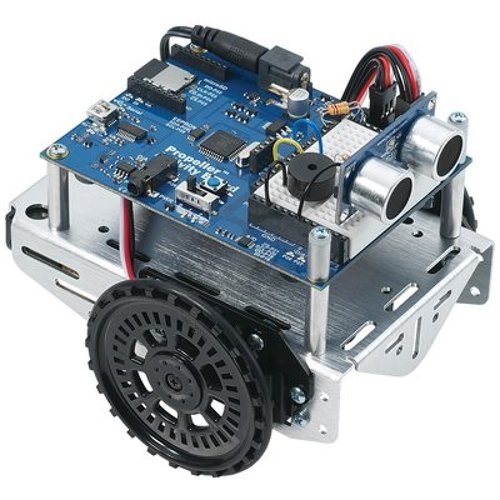
\includegraphics[width=0.4\textwidth]{immagini/robot}
	\caption{Robot utilizzato.}
	\label{fig:robot}
\end{figure}

L'obiettivo finale è quello di far seguire al robot un tracciato disegnato con del nastro isolante di colore nero. Il percorso prevede rettilinei, curve paraboliche, curve ad angolo retto e per finire incroci.

\section{Metodi}

In fisica lo spettro elettromagnetico indica l'insieme di tutte le possibili frequenze delle radiazioni elettromagnetiche. Pur essendo lo spettro continuo, è possibile una suddivisione puramente convenzionale ed indicativa in vari intervalli o bande di frequenza (Figura \ref{fig:spettro})

\begin{figure}[h]
	\centering
	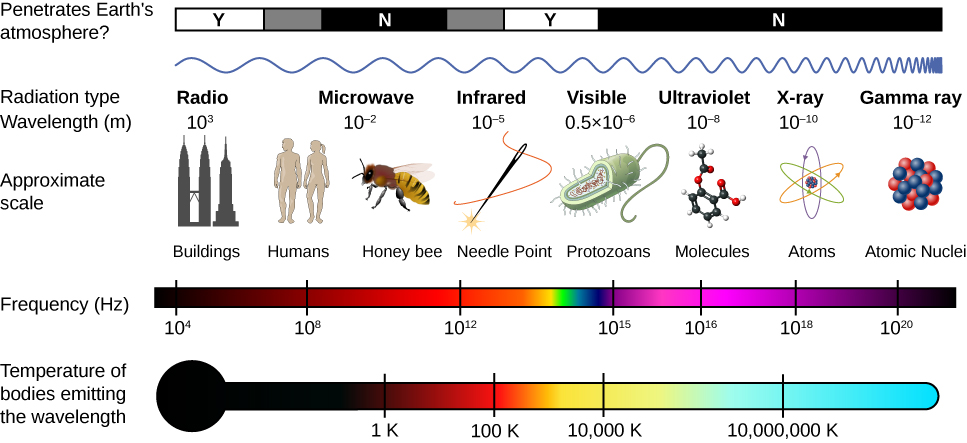
\includegraphics[width=0.45\textwidth]{immagini/spettro}
	\caption{Spettro Elettromagnetico}
	\label{fig:spettro}
\end{figure}

In particolare la radiazione infrarossa (IR) è la radiazione elettromagnetica con banda di frequenza dello spettro elettromagnetico inferiore a quella della luce visibile, ma maggiore di quella delle onde radio, ovvero lunghezza d'onda compresa tra 700 nm e 1 mm (banda infrarossa).
L'infrarosso è utilizzato comunemente come mezzo di trasmissione dati: nei telecomandi dei televisori (per evitare interferenze con le onde radio del segnale televisivo), tra computer portatili e fissi, palmari, telefoni cellulari, nei sensori di movimento e altri apparecchi elettronici. La radiazione infrarossa è soggetta al seguente fenomeno: viene assorbita da un materiale di colore nero e riflessa da uno bianco. 

In elettronica esistono sensori in grado sia di emettere che ricevere il segnale infrarosso. In questo progetto sono stati utilizzati congiuntamente. In particolare sono stati affiancati e tra di loro è stato posto un materiale di colore nero (Figura \ref{fig:coppia}), il cui scopo è quello di evitare che la radiazione infrarossa emessa dall'emettitore venga rilevata dal ricevitore abbinato.

\begin{figure}[h]
	\centering
	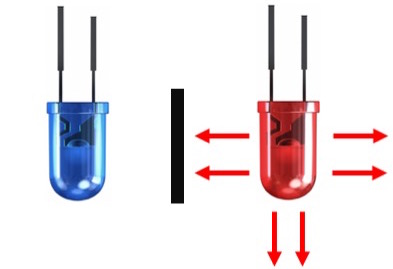
\includegraphics[width=0.35\textwidth]{immagini/coppia}
	\caption{Il led di colore rosso è l'emettitore. Il led di colore blu è il ricevitore.}
	\label{fig:coppia}
\end{figure}

Questa configurazione permette di distinguere una superficie bianca da un nera. Com'è possibile vedere in figura \ref{fig:leds_absorb1}, la coppia di componenti è stata posizionata in prossimità di una superficie bianca. La radiazione infrarossa, che ha origine dall'emettitore, viene riflessa dalla superficie. Ai capi del ricevitore, un dispositivo analogico, è possibile misurare una tensione direttamente proporzionale alla quantità di raggi infrarossi che il sensore riceve. In questo caso quindi tale tensione sarà sicuramente maggiore di zero.

\begin{figure}[h]
	\centering
	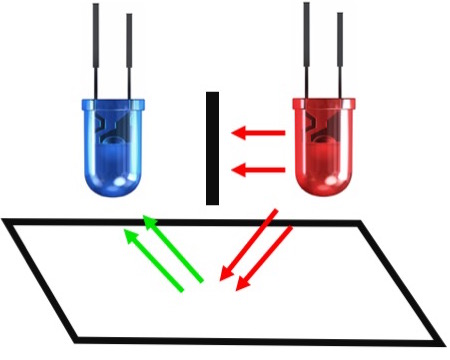
\includegraphics[width=0.35\textwidth]{immagini/leds_absorb1}
	\caption{Superficie bianca}
	\label{fig:leds_absorb1}
\end{figure}

\newpage
Viceversa, se la coppia di componenti si trova in prossimità di una superficie nera, come in figura  \ref{fig:leds_absorb2}, quest'ultima assorbirà quasi tutta la radiazione infrarossa e di conseguenza al ricevitore non arriverà nulla Quindi in uscita si leggerà una segnale basso ovvero una tensione vicina allo zero.

\begin{figure}[h]
	\centering
	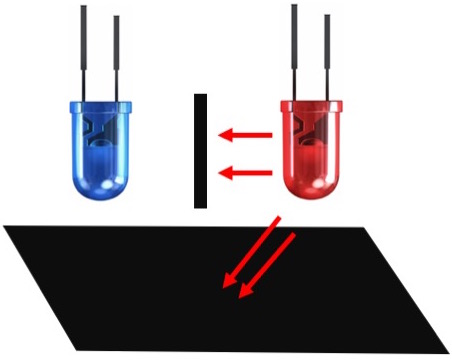
\includegraphics[width=0.35\textwidth]{immagini/leds_absorb2}
	\caption{Superficie nera}
	\label{fig:leds_absorb2}
\end{figure}

In questo lavoro sono state utilizzate tre coppie di sensori/emettitori divise ciascuna da una lunga linea di materiale colorato di nero. Le coppie sono disposte in modo tale da formare una griglia (Figura \ref{fig:configurazione}). La prima fila è composta da tutti i ricevitori mentre la seconda da tutti gli emettitori. 

\begin{figure}[h]
	\centering
	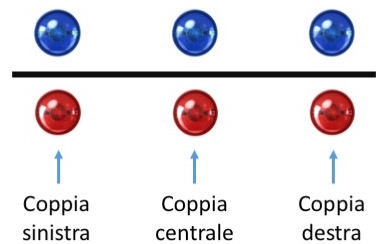
\includegraphics[width=0.35\textwidth]{immagini/configurazione}
	\caption{Griglia formata dalle coppie di ricevitori/emettitori.}
	\label{fig:configurazione}
\end{figure}

D'ora in poi verrà indicata la coppia sinistra con il simbolo $L$, la coppia centrale con $C$ e quella di destra con $R$.
Inoltre ciascun ricevitore di ciascuna coppia è stato collegato all'ingresso analogico del microcontrollore Arduino. Quest'ultimo, con l'impiego di un convertitore analogio-digitale, campiona il segnale continuo e il valore dei quanti varia va da 0 a 1023.

La griglia di sensori è stata montata sullo chassis del robot, in modo tale da trovarsi a 0.5 centimetri da terra (Figura \ref{fig:robot_stilizzato}).   

\begin{figure}[h]
	\centering
	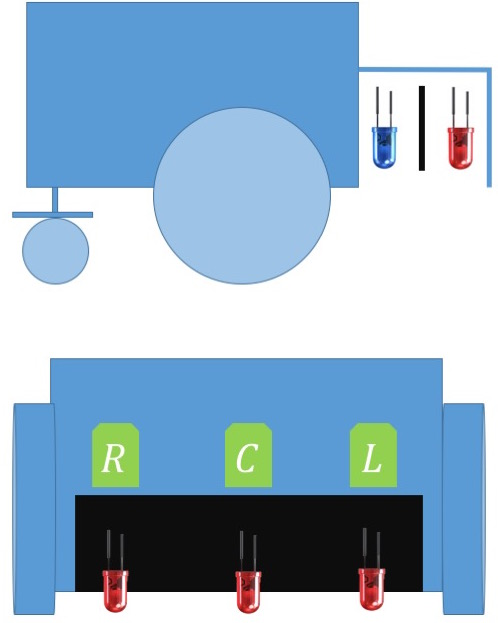
\includegraphics[width=0.3\textwidth]{immagini/robot_stilizzato}
	\caption{Rispettivamente il prospetto laterale e frontale del robot. In quest'ultimo non si vedono i ricevitori infrarossi in quanto coperti dagli emettitori.}
	\label{fig:robot_stilizzato}
\end{figure}

L'obiettivo è quello di mantenere la $C$ perfettamente allineata con una linea nera. Di conseguenza, se questa condizione non si verifica, è stato introdotto il concetto di distanza definito come:

\begin{equation} \label{eq:equazione_errore}
distanza = (R - C) - (L - C)
\end{equation}

L'equazione è stata esposta con un abuso di notazione in quanto $R$, $C$ e $L$ indicano i valori letti dai ricevitori di ciascuna coppia sui quali è stato applicato un filtro complementare e una media. Per comprendere meglio la formula supponiamo che il valore letto dal ricevitore sia pari a 0 se si trova sulla linea nera e pari a 10 se si trova sulla superficie bianca. Supponiamo inoltre di trovarci nella situazione illustrata in figura \ref{fig:t0}
Il ricevitore $C$ leggerà un valore pari a 0 mentre $L$ e $R$ 10. Dall'equazione \ref{eq:equazione_errore} la distanza risulta pari 0 in quanto il robot si trova perfettamente allineato (e di conseguenza anche $C$) alla linea nera.

\begin{figure}[h]
	\centering
	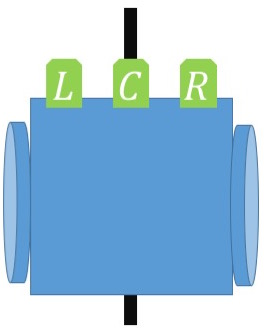
\includegraphics[width=0.3\textwidth]{immagini/t0}
	\caption{}
	\label{fig:t0}
\end{figure}

Nella figura \ref{fig:t1} è illustrato un altro scenario. Il robot non è allineato alla linea nera e quindi se continuasse ad avanzare in quella direzione finirebbe per perdere la linea. Dall'equazione \ref{eq:equazione_errore} la distanza da $C$ è pari a 10, il massimo possibile. Nel caso in cui il robot si trovasse con $R$ sulla linea nera e $L$ e $C$ sulla superficie bianca (ovvero lo scenario speculare rispetto alla figura \ref{fig:t1}) la distanza risultante sarebbe pari a -10. Il segno positivo o negativo discrimina quindi le due condizioni tra loro simmetriche.

\begin{figure}[h]
	\centering
	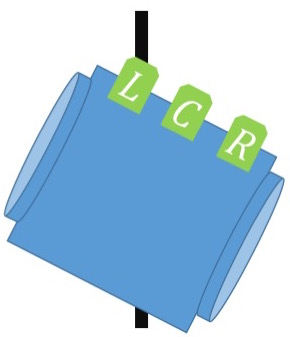
\includegraphics[width=0.3\textwidth]{immagini/t1}
	\caption{}
	\label{fig:t1}
\end{figure}


Nella figura \ref{fig:t2} il robot deve affrontare un incrocio. Tutti i ricevitori forniscono come valore di riferimento 0. La distanza di conseguenza è 0 ($C$ è allineato con la linea nera) e quindi il robot procede sulla stessa direzione.

\begin{figure}[h]
	\centering
	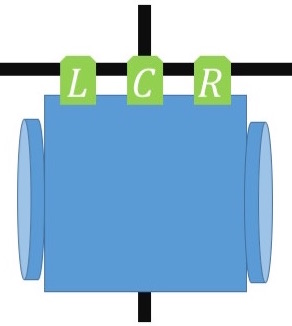
\includegraphics[width=0.3\textwidth]{immagini/t2}
	\caption{}
	\label{fig:t2}
\end{figure}

Nella figura \ref{fig:t3} è illustrato l'ultimo scenario che il robot può affrontare, ovvero una curva a 90 gradi. La distanza risultante dall'equazione \ref{eq:equazione_errore} è pari a 10. Nel caso di curva a destra, il caso è simmetrico in quanto la distanza è pari a -10.

\begin{figure}[h]
	\centering
	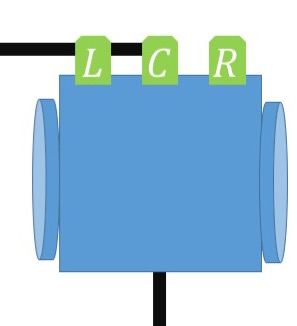
\includegraphics[width=0.3\textwidth]{immagini/t3}
	\caption{}
	\label{fig:t3}
\end{figure}


La distanza calcolata con l'equazione \ref{eq:equazione_errore} viene dato in ingresso ad un controllore PID.

Il controllore \textbf{PID (Proportional Integral Derivative Controller)} è un sistema in retroazione negativa ampiamente impiegato nei sistemi di controllo. Il controllore acquisisce in ingresso un valore da un processo e lo confronta con un valore di riferimento. La differenza, il cosiddetto segnale di errore, viene quindi utilizzata per determinare il valore della variabile di uscita del controllore, che è la variabile manipolabile del processo.

Il PID regola l'uscita in base a:
\begin{enumerate}
	\item il valore del segnale di errore (azione proporzionale);
	\item i valori passati del segnale di errore (azione integrale);
	\item quanto velocemente il segnale di errore varia (azione derivativa).
\end{enumerate}

Lo schema di funzionamento del PID è riepilogato  in figura \ref{fig:pid}.

\begin{figure}[h]
	\centering
	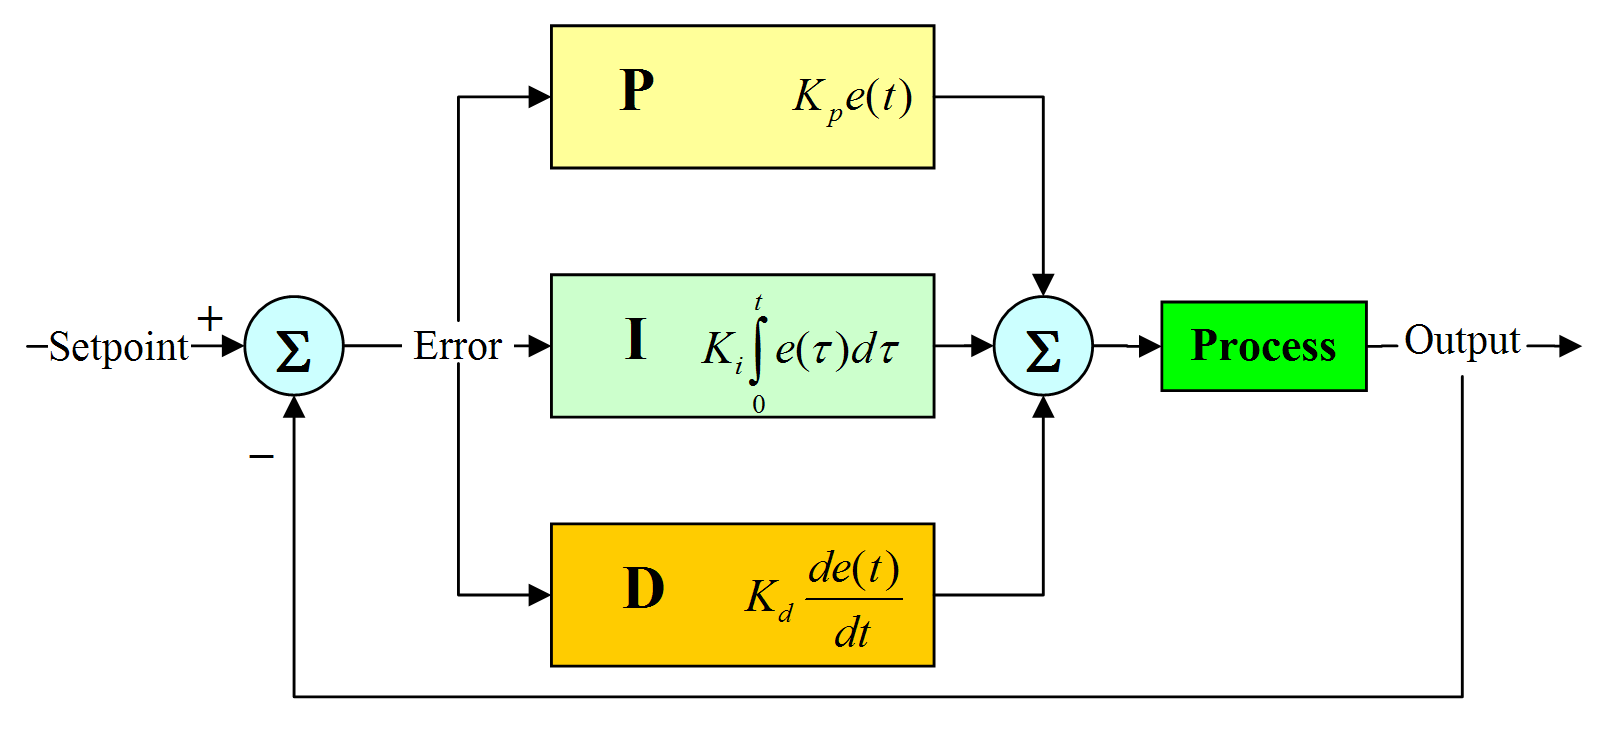
\includegraphics[width=0.5\textwidth]{immagini/PID}
	\caption{}
	\label{fig:pid}
\end{figure}

In questo lavoro il controllo PID è stato utilizzato per riportare la distanza a zero. I parametri del PID sono stati scelti facendo delle prove direttamente sul campo. Inizialmente è stato predisposto un circuito, sulla quale far girare il robot, molto semplice ovvero senza curve a 90 gradi o incroci. Quanto il robot è stato in grado girare su questo tracciato si è passato ad uno più complesso. Anche in questo caso i valori del PID sono stati perfezionati fin quando il robot non è riuscito a completare il circuito.

Il robot per muoversi utilizza due servomotori a rotazione continua. Questi si presentano come piccoli contenitori di materiale plastico da cui fuoriesce un perno in grado di ruotare (Figura \ref{fig:servo}). 

\begin{figure}[h]
	\centering
	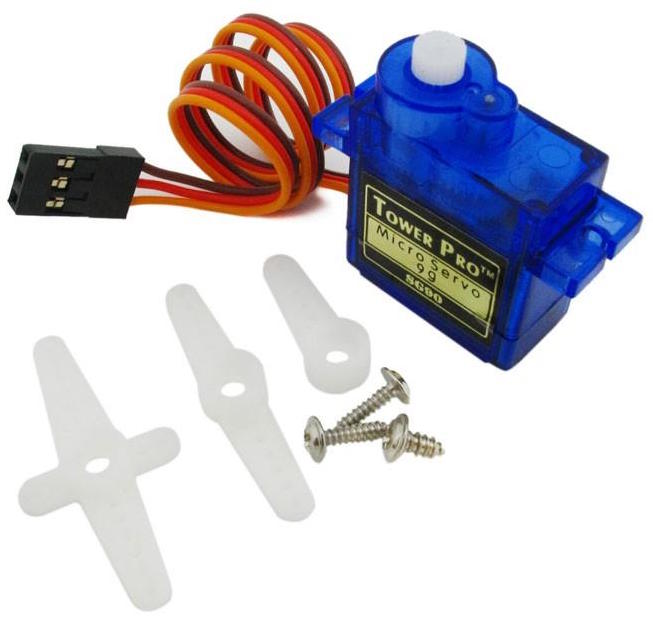
\includegraphics[width=0.35\textwidth]{immagini/servo}
	\caption{}
	\label{fig:servo}
\end{figure}

I tre fili del motore devono essere collegati nel seguente modo: il rosso all'alimentazione (5 Volt), il nero alla terra (Ground) e l'arancione ad un porta di Arduino che supporta il Pulse With Modulation (\textbf{PWM}). La libreria di Arduino \textit{Servo.h} permette un utilizzo dei motori molto semplice attraverso un interfaccia estremamente comoda. Una volta dichiarata la variabile di tipo \textit{Servo}, attraverso la funzione \textit{attach(int port)} si crea il riferimento tra il numero di porta e la variabili stessa. A questo punto con la funzione \textit{write(int speed)} si impartisce al servo la velocità di rotazione. Il parametro \textit{int speed} può assumere valori tra 0 e 180. In particolare se \textit{speed} è uguale a 0 il servo ruota alla velocità massima in un senso; se uguale a 90 il motore non ruota e infine per 180 la velocità di rotazione è massima ma nel senso opposto. 

I motori che sono stati utilizzati non sono però perfettamente calibrati in quanto per fermare la rotazione bisogna porre \textit{speed} pari a 89 anziché 90. Questa ha un valore di partenza impostato a 98 per il motore destro e 88 per il sinistro. In tal modo entrambi ruotano alla stessa velocità e nello stesso verso. A questo punto per controllare il robot viene aggiunto il valore restituito dal PID diviso per due e arrotondato. 

\section{Risultati}

Il robot è in grado di seguire la linea in tutte le condizioni discusse nella sezione precedente. Per questo motivo è stata aumentata la velocità ovvero il parametro \textit{speed} è stato portato a 102 per il motore destro e 84 per il sinistro. Con questa configurazione però il robot è grado di eseguire le curve di 90 a sinistra ma non quelle a destra. Indagando questo strano fenomeno è venuto fuori che i motori non si comportano allo stesso modo. Infatti a parità di \textit{speed} la velocità di rotazione è differente. Questa problema si accentua aumentando appunto la velocità. Per risolvere l'inconveniente si è tentato di introdurre parametri di correzione sul software. L'esito però è stato negativo in quanto l'effettiva variazione di velocità rispetto alla variazione di \textit{speed} è non lineare. L'unico modo per risolvere il problema è stato quello di tornare alla velocità iniziale.

\section{Sviluppi Futuri}

Grazie all'esperienza maturata con questo progetto in futuro sarebbe interessante sviluppare una nuova versione del Line Follower. A livello hardware sarebbe interessante passare da servo motori a rotazione continua a motori DC. Questi ultimi permettono una maggiore velocità anche se sono più complicati da gestire in quanto richiedo una shield apposita per il loro controllo e alimentazione.
A questo punto sarebbe interessante inviare la telemetria del robot (valori restituiti dai ricevitori infrarossi, valore restituito dal PID e così via). Questo permetterebbe di avere dati in tempo reale su cui lavorare e di conseguenza poter migliorare ulteriormente i parametri del PID e il software di controllo in generale.
Per finire la ruota non snodata fornita con lo chassis dovrebbe essere modificata per evitare fastidiosi attriti che potrebbero verificarsi aumentando la velocità.

\end{document}
